\documentclass{article}

\usepackage{proposal}
\usepackage{float}
\newcommand{\tb}[1]{\textbf{#1}}
\newcommand{\mb}[1]{\boldsymbol{#1}}
\newcommand{\ora}[1]{\overrightarrow{#1}}
\newcommand{\ola}[1]{\overleftarrow{#1}}

\setproposaltitle{Machine Comprehension}
\def\*#1{\mathbf{#1}}
\def\ab{ab}
\addauthor{Divyansh Singhvi}{150238}
\addauthor{Megha Agarwal}{150403}
\addauthor{Saransh Bhatnagar}{150637}
\addauthor{Siddhant Garg}{150711}
\addauthor{Dushyant Kumar}{150242}

\begin{document}
\makeheader

\rabstract{
	Machine Comprehension is a fundamental problem in Natural Language. A recently released dataset, the Stanford Question Answering Dataset (SQuAD), offers a large number of real questions and their answers created by humans through crowdsourcing. SQuAD provides a challenging testbed for evaluating machine comprehension algorithms, partly because compared with previous datasets, in SQuAD the answers do not come from a small set of candidate answers and they have variable lengths. In this project we implemented two models First we implemented Match-LSTM model using answer pointer using boundary model. Then we also implemented another model based on Scaled-Dot Product Attention and Multi-Head Attention. The later model gives better results.
}

\begin{psection}{Introduction}

	\sloppy
	Question Answering (or Machine Comprehension) is a fundamental problem in Natural Language Processing where we want the computer system to be able to understand a corpus of human knowledge and answer questions provided in Natural Language.
	This involves seemingly simple, but complex tasks such as understanding human language enough to interpret provided questions, and searching for an appropriate answer.

	A distinguishing characteristic between humans and naive models is the ability of humans to quickly relate the passages to focus on subsets of the passage with demarcating words related to the task at hand.
	And to solve this problem Attention mechanism is used which allows modeling of dependencies without regard to their distance in the input or output sequences.

	There have been many approaches to solving the machine comprehension, however most lack the scalability and the lightness of the model. In our project, we intend to explore the high maintenance characteristic of these models and incorporate

	In this work we propose the Match-LSTM based on clustering of question type which optimizes the choice of hyper parameters and subsequently also modelled a different architecture for Q\&A based on Multi-Head attention. Further, to deal with the challenge of varying answer length Answer Pointer technique is incorporated in the output layer.

\end{psection}

\begin{psection}{Problem Statement}

	In this course project, we aim to explore the problem of Machine Comprehension (or Question Answering) by using Deep Learning based models and see how they perform on the Stanford Question Answering Dataset (SQuaD).

	We state our problem statement similar to as stated in \citep{squad}.

	For each question-passage-answer tuple $(\vQ, \vP, \vA)$, where $\vQ = (q_1 \dots q_M)$ are the tokens for the question, $\vP = (p_1 \dots p_N)$ are the tokens for the passage, and $\vA = (a_b, a_e)$ is the answer span, $a_b$ and $a_e$ representing the beginning and ending indices in the passage.
	The task is maximising the conditional probability $\prob{\vA = (a_b, a_e) \pipe \vQ, \vP}$, \ie the probability of answer being correct, given the question and the passage or instead estimating $\prob{\vA \pipe \vQ, \vP}$ and thereby finding the answer
	\begin{align*}
		\vA^\ast = \argmax{\vA} \prob{\vA \pipe \vQ, \vP}.
	\end{align*}

\end{psection}

\begin{psection}{Dataset}

	We have used the SQuAd \citep{squad} dataset, for the goal of studying techniques in Machine Comprehension.

	The Stanford Question Answering Dataset (SQuAD) is a reading comprehension consisting of 100,000+ question-answers corresponding to passages extracted from over 500 wikipedia articles, where the answer to each question is a continuous segment of text from that passage.

	The dataset is roughly portioned in 80k test set, 10k training set and 10k validation set.
	SQuAD does not provide a list of answer choices for each question, as compared to other datasets.
	Also, unlike some other contemporary datasets whose questions and answers are created automatically in cloze style, the question and answers in SQuAD were created by humans through crowdsourcing making the dataset more realistic.

	Another difference between SQUAD and cloze style queries is that answers to cloze style queries are single words or entities while answer in SQuAD can be non-entities and can contain long phrase.

	In order to understand the dataset in more detail and motivate further design and hyper parameter decision, We perform some basic analysis on the dataset in the form of histograms of the context length, question length, and the answer length in the training set.

	\begin{figure}[H]
			\centering
			\begin{minipage}{0.47\textwidth}
				\centering
				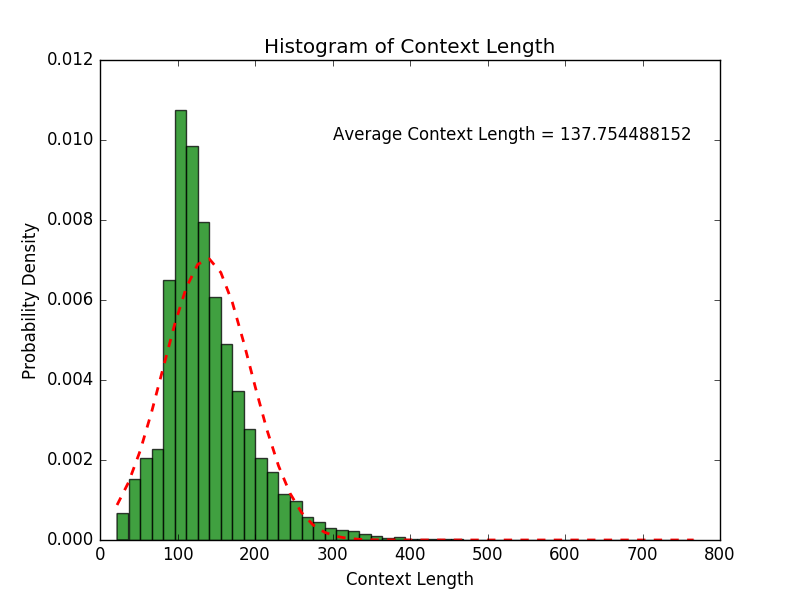
\includegraphics[height=135px]{includes/context_hist_fin.png}
				\caption{}
			\end{minipage}
			\begin{minipage}{0.47\textwidth}
				\centering
				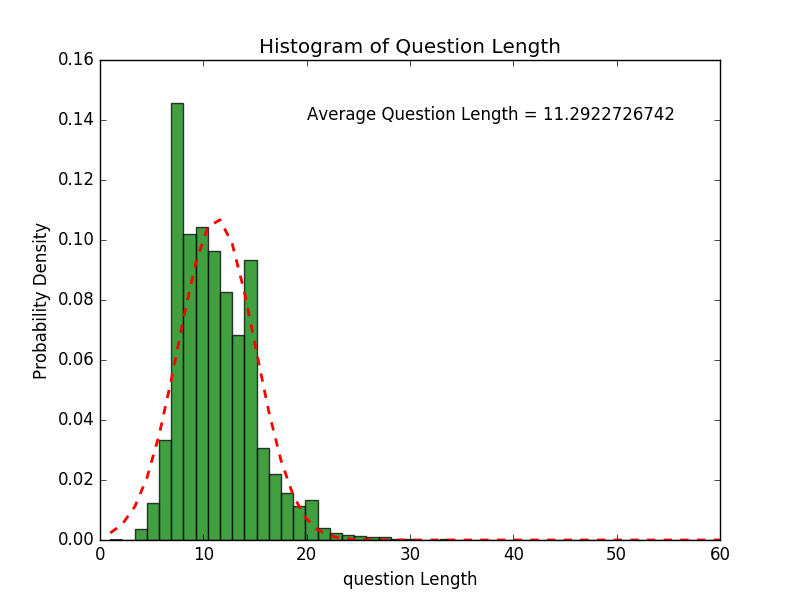
\includegraphics[height=135px]{includes/question_hist_fin.png}
				\caption{}
			\end{minipage}
	\end{figure}
	\begin{figure}[H]
	\centering
			\begin{minipage}{0.47\textwidth}
				\centering
				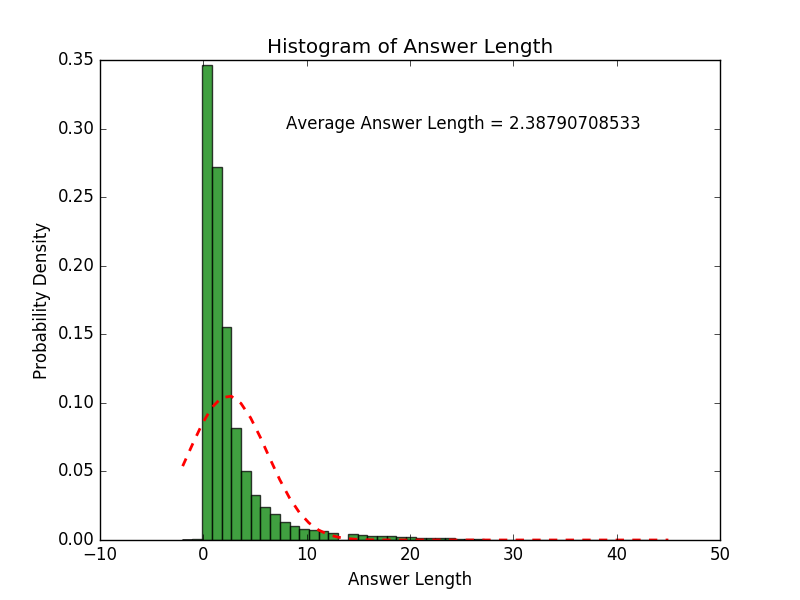
\includegraphics[height=135px]{includes/ans_hist_fin.png}
				\caption{}
			\end{minipage}
			\begin{minipage}{0.47\textwidth}
				\centering
				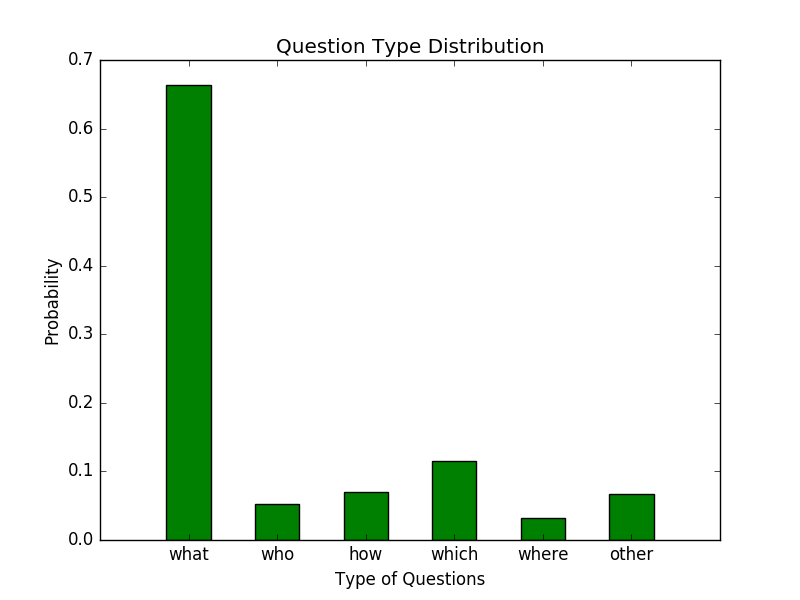
\includegraphics[height=135px]{includes/dist2.png}
				\caption{}
			\end{minipage}
% 			\caption{Working of a simple LSTM. \et{\citep[Source:][]{lstm-blog}}}
% 			\label{fig:lstm-flow}
		\end{figure}

	From the histogram of context lengths(Figure 1), the majority of context are shorter than 300 words. Hence it is possible to set the maximum context length to around 300 without losing to much information but gaining a lot in terms of memory and speed efficiency. The maximum question length can be set to 30 and maximum answer length of 10 words in the same way.

	The histogram for answer lengths(Figure 2) show that the majority of answers are less than 10 words. This helps us determining answer span at test time as we could limit the search for answer span less than 10 words thus preventing model to predict unnecessarily long span.

	We also examine the distribution of different question types like 'what', 'who', 'how', 'which', 'where', and other type include 'when' and 'why' type question. As we can see from the graph(Figure 4) 'what' type question account for largest proportion in dataset.

	In additon, the span-based QA setting is quite natural.
	For many user questons into search engines, open-domain QA systems are often able to find the right documents that contain the answer.
	The challenge is the last step of ``answer extracton'', which is to find the shortest segment of text in the passage or document that answers the question \footnote{\url{https://rajpurkar.github.io/mlx/qa-and-squad/}}.

\end{psection}

\begin{psection}{Relevant Background}

	\begin{psubsection}{Long Short Term Memory}
		Long Short Term Memory \citep[LSTM,][]{lstm} networks are a special kind of Recurrent Neural Networks (RNNs), capable of learning long-term dependencies.
		LSTMs are explicitly designed to avoid long-term dependency problem, for example, for predicting a word after observing a sequence of words history, we might need the context of the words observed much before the `to be predicted' word.

		\sloppy
		This requires a memory model, which vanilla RNNs are incapable of handling. Remembering information for long periods of time is default behavior of the LSTM networks, which is handled using states and the controlling the flow of information is handled using gating networks. LSTMs, therefore, have the ability to remove or add information to the cell state, regulated by gates or gated networks.
% 		The structure of a simple LSTM network is given in Figure \ref{fig:lstm}

% 		\begin{figure}[ht!]
% 			\centering
% 			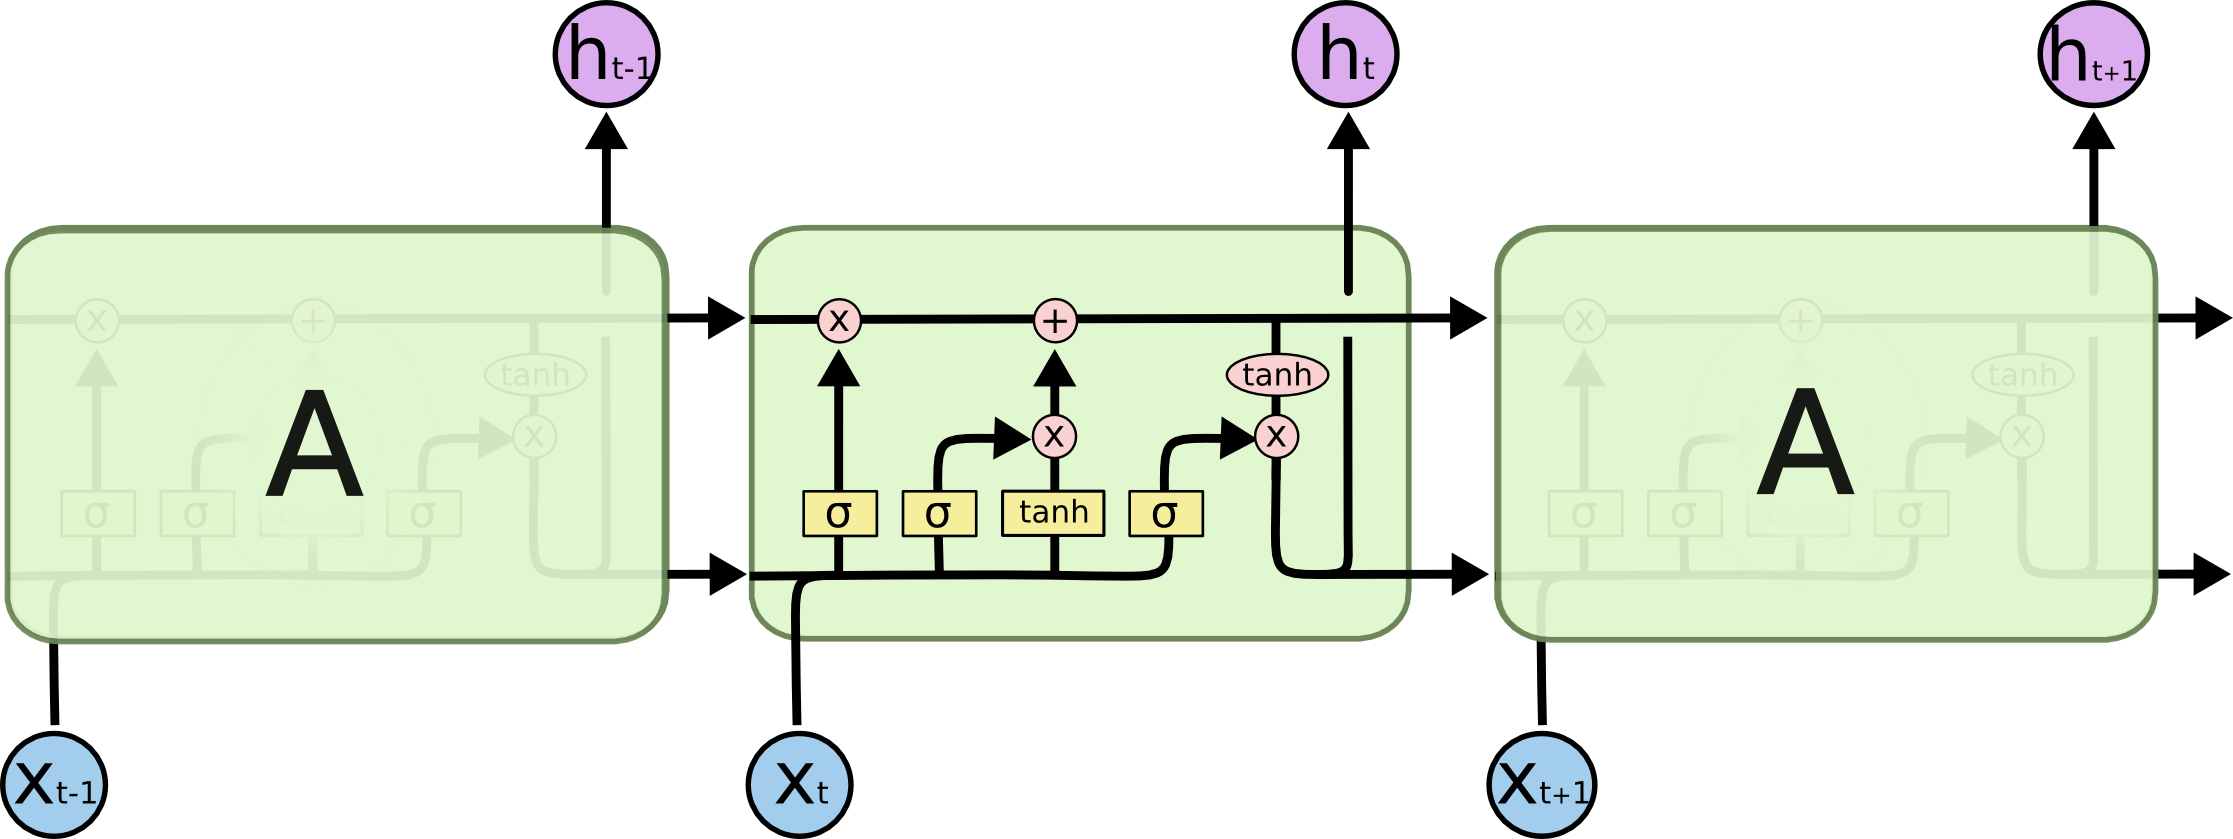
\includegraphics[width=0.8\textwidth]{includes/lstm-chain.png}
% 			\caption{Insides of a LSTM Network. \et{\citep[Source:][]{lstm-blog}}}
% 			\label{fig:lstm}
% 		\end{figure}

		\begin{pssubsection}{Bidirectional LSTMs}
			Bidirectional RNNs \citep[BRNNs,][]{rnn-blog}, which are the base of bidirectional LSTMs, are based on the idea that the output at time $t$ may not only depend on the previous elements in the sequence, but also future elements, for example, word prediction, such as filling in a blank within a sentence, might benefit from including the post blank words into consideration while prediction the current word.

			Bidirectional RNNs, in their essence, are just two RNNs stacked on top of each other.
			The output is then computed based on the hidden state of both RNNs.
			Combing BRNNs with LSTM gives bidirectional LSTM which can access long-range context in both input directions.

% 			\begin{figure}[ht!]
% 				\begin{minipage}{0.47\textwidth}
% 					\centering
% 					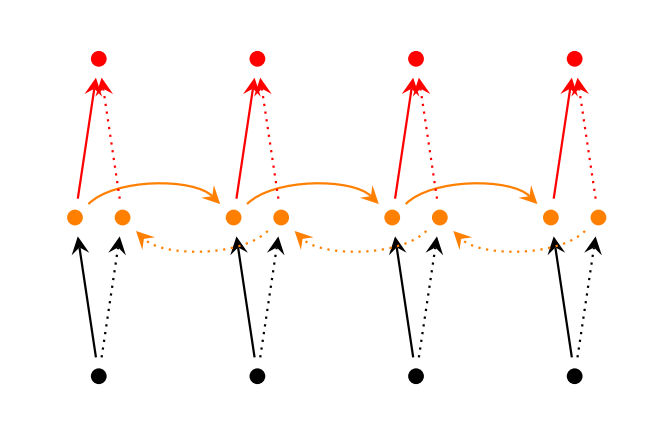
\includegraphics[width=200px]{includes/bidirectional-rnn.png}
% 					\caption*{(a) Bidirectional RNN}
% 				\end{minipage}
% 				\begin{minipage}{0.47\textwidth}

% 					\centering
% 					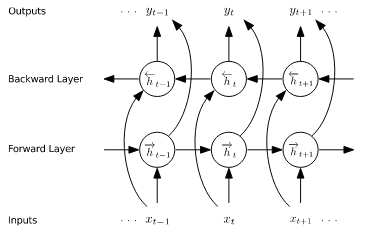
\includegraphics[width=200px]{includes/bidirectional-lstm.png}
% 					\caption*{(b) Bidirectional LSTM}
% 				\end{minipage}
% 				\caption{Biderectional RNNs (left) and LSTMs (right) \et{\citep[Source:][]{rnn-blog}}}
% 			\end{figure}

		\end{pssubsection}

		\begin{pssubsection}{Match-LSTM}

			Match-LSTMs \citep{match-lstm} are an extension to basic LSTMs, introduced by \et{Wang and Jiang} for the purpose of textual entailment, and later used the same in machine comprehension to achieve state-of-the-art results on the SQuAD (at the time of publication).

			Match-LSTM attempts to recover an sequence of positions within a context paragraph using the contents of the context and an associated question \citep{match-lstm-m}.

			To verify textual entailment, match-LSTM goes through the tokens of the hypothesis sequentially. And for each position, attention mechanism is used to obtain a weighted vector representation of the premise. This weighted premise combined with current token of hypothesis fed into match-LSTM.

			\sloppy
			The match-LSTM model essentially sequentially aggregates the matching of the attention weighted premise to each token of the hypothesis and uses the aggregated matching result to make a final prediction.

			Details of the model are given in the papers \cite{match-lstm} and \cite{match-lstm-mc}

		\end{pssubsection}

		\begin{psubsection}{Attention Mechanism}
		Most of the sequence transduction models comprise of encoder-decoder configuration that are based on complex recurrent or convolutional neural networks. However, The efficiency and model performance can be boosted through adding attention mechanism between encoder and decoder layers.


		In the case of machine comprehension, attention mechanism involves creating an attention weighted representation of the context using the question as the test and correspondingly comprehension as hypothesis. The attention weighted context representation acts as input for decoder and subsequently the pointer network also uses the same attention mechanism to compute the probabilistic expected answer tokens to the query.
		\end{psubsection}

	\end{psubsection}

\end{psection}

\begin{psection}{Previous Works}

	Traditional solutions question answering tasks relied on NLP pipelines that involved multiple steps of linguistic and lexical analysis, including syntactic parsing, named entity recognition, question classification, semantic parsing, etc.
	In these approaches each layer of parsing added its own set of errors or loss which propogated over pipelines to subtle failures that required a lot of manual tweaking to get to the right results.

	Existing end-to-end neural models assume that the answer is a single token making them unsuitable for use in SQuAD, which expects a sequence based answers. Hence, we require new and more advanced models for machine comprehension tasks. We have described a few of them below.

	Most of the state-of-the-art approaches have the following settings in common, which we, as well, did extend in our approach as an attempt to solve the problem of question answering in SQuAD.

	\begin{enumerate}
		\item Pre trained GLoVe \citep{glove} vectors are used as embeddings for each word, therefore forming the word embedding layer.

		\item This word embedding layer is connected through LSTM which could of different types like vanilla LSTM, bidirectional LSTM, match-LSTM, etc. to develop a context based embedding layer.

		\item \sloppy
		    This layer is followed by attention flow layer which is used to make the model aware of the query.
			The paragraph and query are both processed through the attention mechanism to generate an interdependent context, therefore learning a query aware latent representing of the passage.

		\item This latent representation is therefore used to predict the answer spans using various strategies, some of which we discuss briefly in the following sections.
	\end{enumerate}

% 	\begin{psubsection}{Bi-Directional Attention Flow for Machine Comprehension}

% 		The BiDAF \citep{bidaf} model is a hierarchical multi-stage process which consists of six layers. The comprehensive model is given in Figure \ref{fig:bidaf}.

% 		\begin{enumerate}[label=\bt{\theenumi.}]
% 			\ditem[Character Embedding Layer.] Character embedding layer is responsible for mapping each word to a high-dimensional vector space.
% 			We obtain the character-level embedding of each word using Convolutional Neural Networks (CNN) \citep{Char_embedding}.

% 			\ditem[Word Embedding Layer.] Word embedding layer also maps each word to a high-dimensional vector space.
% 			Pre-trained GloVe vectors, are used to obtain the fixed word embedding of each word.

% 			\ditem[Contextual Embedding Layer.] This layer model the temporal interactions between words.
% 			For this, LSTM is placed in both directions and concatenate the outputs of the two LSTMs, thus obtaining \bt{H} from context word vectors $\vX$ and $\vU$ from query word vectors $\vQ$.

% 			\ditem[Attention Flow Layer.] Attention flow layer is responsible for linking information from context and query words.
% 			The inputs to the layer are contextual vector representations of the context $\vH$ and the query $\vU$.
% 			The outputs of the layer are the query-aware vector representations of the context words, $\vG$, along with the contextual embeddings from the previous layer. Shared similarity matrix, $\vS$ is used to obtain the attentions and the attended vectors in both direction.

% 			The similarity matrix $\vS$ is used to obtain the attentions and the attended vectors in both direction, \ie \et{Context-to-Query} Attention and \et{Query-to-Context} Attention.

% 			\ditem[Modeling Layer.] The input to the modeling layer is $\vG$, which encodes the query-aware representations of context words by using two layered bi-directional LSTM.

% 			The output of the modeling layer captures the interaction among the context words conditioned on the query.
% 			The output of the modelling layer is $\vM$.

% 			\ditem[Output Layer.] This layer predict the start and the end indices of the phrase in the paragraph to answer the query.
% 			It outputs probability distribution of the start index, $p^1$ over the entire paragraph by using $\vG$ and $\vM$ and predicts the probability distribution of the end index, $p^2$ by using $\vG$ and $M^{2}$, where $M^{2}$ is calculated by passing $\vM$ through another bidirectional LSTM.

% 		\end{enumerate}

% 		\begin{figure}[ht!]
% 			\centering
% 			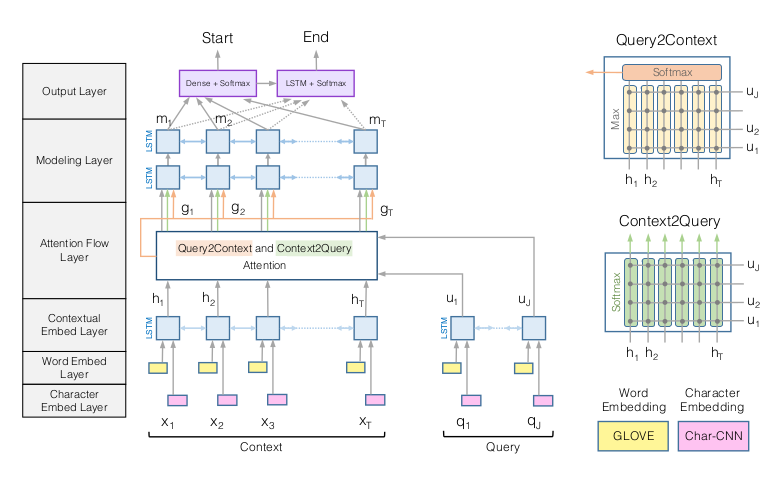
\includegraphics[height=250px]{includes/bidaf.png}
% 			\caption{Bi-Direction Attention Flow Model \et{\citep[Source:][]{bidaf}}}
% 			\label{fig:bidaf}
% 		\end{figure}

% 	\end{psubsection}

	\begin{psubsection}{FastQA}
		The FastQA \citep{fastqa} model consists of three basic layers, namely the embedding, encoding and answer layer. The FastQA model is given in \ref{fig:fqa}

		\begin{enumerate}
			\ditem[Embedding Layer.] It computes the embedding of tokens by concatenating lookup-embedding and char-embedding.

			\ditem[Encoding Layer.] This layer computes the query aware context embedding by concatenating earlier embedding, word-in-question features.
				The word-in-question features determine whether the context words are present in query or not and how similar they are to question tokens.
				Then these query aware context embedding is fed to a bidirectional RNN to allow for interaction between the features accumulated in the forward and back-ward RNN.

			\ditem[Answer Layer.] After encoding context and question tokens, the probability distribution $p_s$ for the start location of the answer is computed by a feed-forward neural network and then the conditional probability distribution $p_e$ for the end location conditioned on the start locations is computed similarly by a feed-forward neural network.

				The overall probability p of predicting an answer span $(s, e)$ is $p(s, e) = p_s(s) \cdot p_e (e|s)$.
				The model is trained to minimize the cross-entropy loss of the predicted span probability $p(s, e)$.
		\end{enumerate}

% 		\begin{figure}[ht!]
% 			\centering
% 			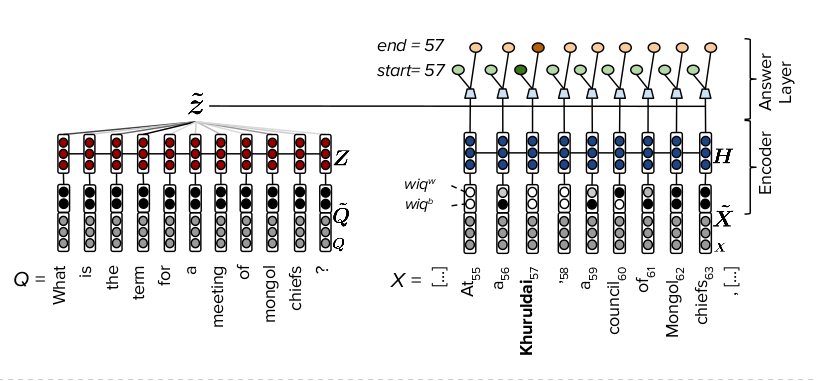
\includegraphics[height=170px]{includes/fast-qa.png}
% 			\caption{Illustration of FastQA system \et{\citep[Source:][]{fastqa}}}
% 			\label{fig:fqa}
% 		\end{figure}

	\end{psubsection}

	\begin{psubsection}{R-Net: Machine Reading Comprehension with Self-Matching Networks}
		R-Net \citep{r-net} is an end-to-end neural network model for reading comprehension and question answering.
		This model consists of four parts:
		\begin{enumerate}
			\item The recurrent network encoder to build representation for questions and passages separately,
			\item the gated matching layer to match the question and passage,
			\item the self-matching layer to aggregate information from the whole passage, and
			\item the pointer-network based answer boundary prediction layer.
		\end{enumerate}

% 		A view on the R-Net model is given in Figure \ref{fig:r-net}.

% 		\begin{figure}[ht!]
% 			\centering
% 			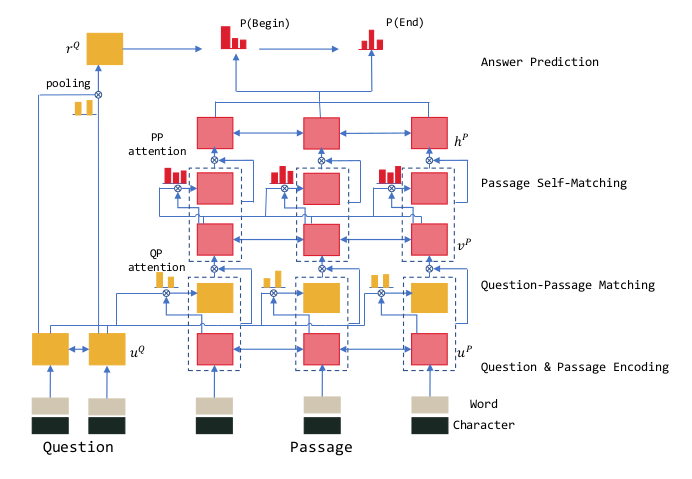
\includegraphics[height=250px]{includes/r-net.png}
% 			\caption{R-NET structure overview \et{\citep[Source:][]{r-net}}}
% 			\label{fig:r-net}
% 		\end{figure}

		\begin{subsubsection}{R-Net Structure}

			\sloppy
			First, the question and passage are processed by a bidirectional recurrent network separately. We then match the question and passage with gated attention-based recurrent networks, obtaining question-aware representation for the passage. On top of that, we apply self-matching attention to aggregate evidence from the whole passage and refine the passage representation, which is then fed into the output layer to predict the boundary of the answer span.

		\end{subsubsection}

		\begin{subsubsection}{Gated Attention Based RNNs}

			A gated attention-based recurrent network is used to incorporate question information into passage representation. It is a variant of attention-based recurrent networks, with an additional gate to determine the importance of information in the passage regarding a question. Different from the gates in LSTM or GRU, the additional gate is based on the current passage word and its attention-pooling vector of the question, which focuses on the relation between the question and current passage word.

		\end{subsubsection}

		\begin{subsubsection}{Self-Matching Attention}

			It is a directly matching the question-aware passage representation against itself. It dynamically collects evidence from the whole passage for words in passage and encodes the evidence relevant to the current passage word and its matching question information into the passage representation. Self-matching extracts evidence from the whole passage according to the current passage word and question information.

		\end{subsubsection}

		\begin{subsubsection}{Output Layer}

			Pointer networks are used to predict the start and end position of the answer. r. In addition, we use an attention-pooling over the question representation to generate the initial hidden vector for the pointer network. Given the passage representation, the attention mechanism is utilized as a pointer to select the start position $p^1$ and end position $p^2$ from the passage.

		\end{subsubsection}

		\sloppy
		The R-Net model is the current state-of-the-art model for machine comprehension on SQuAD. However, we refrain from studying the model due to its complexity and the paper's involved nature.

	\end{psubsection}

	\begin{psubsection}{Question Answering using Match-LSTM and Answer Pointer}

        \cite{match-lstm-mc} introduced the Match-LSTM \citep{match-lstm} model for textual entailment, however, it proved to be useful for the task of machine comprehension as well, with an extra extension using PointerNet \citep{pointernet}. In textual entailment, two sentences are given where one is a premise and the other is a hypothesis. To predict whether the premise entails the hypothesis, the match-LSTM model goes through the tokens of the hypothesis sequentially. At each position of the hypothesis, attention mechanism is used to obtain a weighted vector representation
        of the premise. This weighted premise is then to be combined with a vector representation of the current token of the hypothesis and fed into an LSTM, which we call the match-LSTM. The matchLSTM essentially sequentially aggregates the matching of the attention-weighted premise to each token of the hypothesis and uses the aggregated matching result to make a final prediction.\\
        Detailed analysis and implementation of layers have been discussed in section \ref{match-lstm}.

	\end{psubsection}

	\begin{psubsection}{Comparision of Different Approaches}

		In Table \ref{tab:models}, we have given the EM (Exact Match) and F1 scores \footnote{The description of the scores is given by \cite{squad}}

		\begin{table}[ht!]
			\centering
			\begin{tabular}{l@{\hspace{1em}}|cc|cc}
				\multirow{2}{*}{\bt{Model}}	&	\multicolumn{2}{c|}{\bt{Training Set}}	&	\multicolumn{2}{c}{\bt{Test Set}}	\\
											&	\bt{EM} & \bt{F1}						&	\bt{EM} & \bt{F1}					\\
				\hline
				LR Baseline \citep{squad}	&	40.0 & 51.0								&	40.4 & 51.0							\\
				BiDAF \citep{bidaf}			&	68.0 & 77.3								&	68.0 & 77.3							\\
				FastQA \citep{fastqa}		&	-	 & -								&	68.4 & 77.1							\\
				R-Net \citep{r-net}			&	72.3 & 80.6								&	72.3 & 80.7							\\
				Match-LSTM \citep{match-lstm-mc}	&	64.1 & 73.9						&	64.7 & 73.7							\\
			\end{tabular}
			\caption{Comparision of different models for Machine Comprehension \et{\citep[Source:][]{r-net}}}
			\label{tab:models}
		\end{table}

		\note{The scores are given for single models only, and do not involve ensembles, however for most models, ensembles perform better that single models.}

	\end{psubsection}

\end{psection}

\begin{psection}{\textbf{Our Approaches}}

	In our project, we explored various approaches that have been used for machine comprehension, and analysed the scalability and the performance of each model. The problem with most approaches discussed is the low speed of convergence, given the enormous number of weights in the models.

	Another problem with Match-LSTMs (which R-Net handles efficiently) is that all question types have the same attention mechanism. Subsequently we transformed the proposed model to deal with different types of questions differently, particularly tweaks in the attention mechanism, \ie for different question types, such as `Why?', `What?', etc.
	This is relevant as different question types demand different format of the answers, for example a `Who?' question would focus more on the subject or the object of the sentence. This might increase the performance of the Match-LSTM model, however, will also add to the complexity of the model, and therefore the training time. We now give the details of the Match-LSTM model that we implemented

\begin{psubsection}{Match-LSTM with Answer Pointer}\label{match-lstm}

        We adopted implementation of Match-LSTM and Answer Pointer model proposed by \et{Wang and Jiang}, the architecture consists of three main layers
		\begin{enumerate}[label=\bt{\theenumi.}]
			\ditem[LSTM Preprocessing Layer.]
				The purpose of the \et{LSTM Preprocessing Layer} is to incorporate contextual information into the representation of each token in the passage and the question.
				This is done by passing the passage matrix, $\vP \in \vR^{d \times Q}$ and the question matrix, $\vQ \in \bR^{d \times Q}$ through a one-directional standard LSTM.
				The authors represent this as
				\begin{align*}
					\vH^p	\eq	\overrightarrow{\text{LSTM}}\para{\vP}, \quad\quad
					\vH^q	\eq	\overrightarrow{\text{LSTM}}\para{\vQ}
				\end{align*}
				The matrices $\vH^p$ and $\vH^q$ represent the hidden representations of the passage and the question matrices, respectively.

				\begin{note}
					$Q$ and $P$ are the sizes of or the number of tokens in the question and the passage, respectively
				\end{note}

			\ditem[Match-LSTM Layer.]
				Treating the question as a premise and the passage as the hypothesis, we can apply the Match-LSTM model. At the position $i$, of the passage, the model first uses the standard word-by-word attention mechanism to obtain attention weight-vector $\valpha_i \in \bR^Q$ as follows:
				\begin{align*}
                \boldsymbol{G_i} &= tanh(\*W^q\*H^q + (\*W^p\*h_i^p+\*W^r\*h_{i-1}^r+\*b^p)\otimes e_{\*Q})\\
                \overrightarrow{\alpha_i} & = softmax(\*w^T\overrightarrow{\*G_i}+b\otimes\*e_Q)
            \end{align*}
            where $\*W^q$, $\*W^p$, $\*W^r$, $\in$ $\mathbb{R}^{l\times l}$, $\*b,\*w \in \mathbb{R}^l$ and $\*b \in \mathbb{R}$ are the parameters to be learned. $\overrightarrow{\*h_{i-1}^{r}} \in \mathbb{R}^l$ is the hidden vector at position i-1, and the
outer product (· $\otimes e_Q$) produces a matrix or row vector by repeating the vector or scalar on the left
for Q times.

Essentially, the resulting attention weight $\overrightarrow{\alpha_{i,j}}$ above indicates the degree of matching between the
$i^{th}$ token in the passage with the $j^{th}$ token in the question. The attention weight vector $\alpha_i$ is used to weighted version of the question and combine it with the current token of the passage to form a vector $\overrightarrow{\*z_i}$:
        $$\overrightarrow{\*z_i} =
            \begin{bmatrix}
                \*h_i^p \\ \*H^q\overrightarrow{\alpha_i}^T
            \end{bmatrix}
        $$

        This vector $\overrightarrow{\*z_i}$ is fed into a standard one-directional LSTM to form our so-called match-LSTM:
        $$\overrightarrow{\*h_i^r} = \overrightarrow{\text{LSTM}}(\overrightarrow{\*z_i},\overrightarrow{\*h_{i-1}^r}),$$
        where $\overrightarrow{\*h_i^r}\in \mathbb{R}^l$.

        A Similar Match-LSTM layer is build in the reverse direction. The purpose is to obtain a representation that encodes the contexts from both directions for each token in the passage. To build this reverse match-LSTM, we first define

        \begin{align*}
             \overleftarrow{\*G_i} &= tanh(\*W^q\*H^q + (\*W^p\*h_i^p + \*W^r\overleftarrow{h}_{i+1}^r\*b^p)\otimes \*e_Q),\\
             \overleftarrow{\alpha_i} & = softmax(\*w^T\overleftarrow{\*G_i}+b\otimes \*e_Q),
        \end{align*}
        where the parameters are $(\*W^q,\*W^p,\*W^r,\*b^p,\*w \ and \ b)$
        $\*z_i$ and $\*h_i$ are defined in similar manner.

        Let $\overrightarrow{\*H^r} \in \mathbb{R}^{l\times P}$represents the hidden states $[\overrightarrow{\*h_1^r},\dots,\overrightarrow{\*h_P^r}]$. Similarly $\overleftarrow{\*H^r}\in \mathbb{R}^{l\times P}$ represents $[\overleftarrow{\*h_1^r},\dots,\overleftarrow{\*h_P^r}]$. Define $\*H^r \in \mathbb{R}^{2l \times P}$ as the concatenation of the above two:
        $$\*H^r = \begin{bmatrix}
        \overrightarrow{\*H^r}\\ \overleftarrow{\*H^r}
        \end{bmatrix}$$

		This attention is iteratively used to estimate the bidirectional hidden representation of the passage, which in turn is used to compute the attention itself.
		This iterative procedure ensures that the representation we have for the passage is query aware, and is built using the attention obtained from the query (question).
		This representation is denoted by the matrix $\vH^r$

			\ditem[Answer Pointer Layer.]
				The final layer is the \et{Answer Pointer Layer}, which uses the idea of Pointer Networks \cite{pointernet}.
				This model takes in, as input, the hidden representation $\vH^r$, and tries to identify the answer within the passage using two approaches, the \et{sequence model}, which tries to determine the complete sequence and probabilistically models the whole sequence, and the \et{boundary model}, which is only concerned with the starting and ending tokens of the answer. However, we are only interested in the boundary approach, as it performs better, and better suits the nature of PointerNets.

				The passage (hidden representation $\vH^r$) is first passed through the attention mechanism to compute a attention vector $\vbeta_k \in \bR^{P + 1}$,

			    \begin{align*}
                          \boldsymbol{F}_k &= \text{tanh} \left(\textbf{V} \textbf{H}^r + (\textbf{W}^a \boldsymbol{h}_{k - 1}^a + \boldsymbol{b}^a) \otimes \boldsymbol{e}_P \right) \\
                          \beta_k &= \text{softmax} \left( \boldsymbol{b}^\text{T} \boldsymbol{F}_k + c \otimes \boldsymbol{e}_P \right)
                \end{align*}
			Where $\boldsymbol{h}_{k - 1}^a$ represents the last hidden state of the answer pointer, projections and parameter matrices dimensions are given by $\textbf{H}^r \in \mathbb{R}^{2l\times(P+1)}, \textbf{V} \in \mathbb{R}^{l\times 2l}, \boldsymbol{W}^a \in \mathbb{R}^{l \times l}, \textbf{b}^a, \textbf{v} \in \mathbb{R}^l \text{ and } c \in \mathbb{R}$.\\
			$\beta_{j, k}$ is the probability of selecting the $j$\tth passage token as the $k$\tth token in the answer. The probability of the answer is then modelled as
				\begin{align*}
					\prob{\va \pipe \vH^r}	\eq	\prob{a_s \pipe \vH^r} \prob{a_e \pipe a_s, \vH^r}
				\end{align*}
				where
				\begin{align*}
					\prob{a_k = j \pipe a_1, a_2 \dots a_{k - 1}, \vH^r}	\eq	\beta_{j, k}
				\end{align*}
				Hence, the objective is to maximize $\prob{\va \pipe \vH^r}$, and the answer corresponding to the maximum answer is reported as the answer to the query.
		\end{enumerate}

		Although the Match-LSTM model works well, the problem with this approach (rather problem with using PointerNets) is that answers which are long, \ie have relatively more number of tokens, are predicted with lesser accuracy. However, one of the key benefits of using Match-LSTM is that it is a simpler model (lesser model complexity) than the other state-of-the-art models, and therefore, might be more scalable than other models.


		\ditem[Modifications in Answer Pointer Layer]
		       In order to differentiate the question types i.e.\ - what? where? why? how? etc., we setup different Answer Pointer layers for different question types.
		       Training the model based on the clusters on query level allows us to modify the hyper parameters to increase the efficiency of the model.

	\begin{figure}[ht!]
				\begin{minipage}{0.47\textwidth}
					\centering
					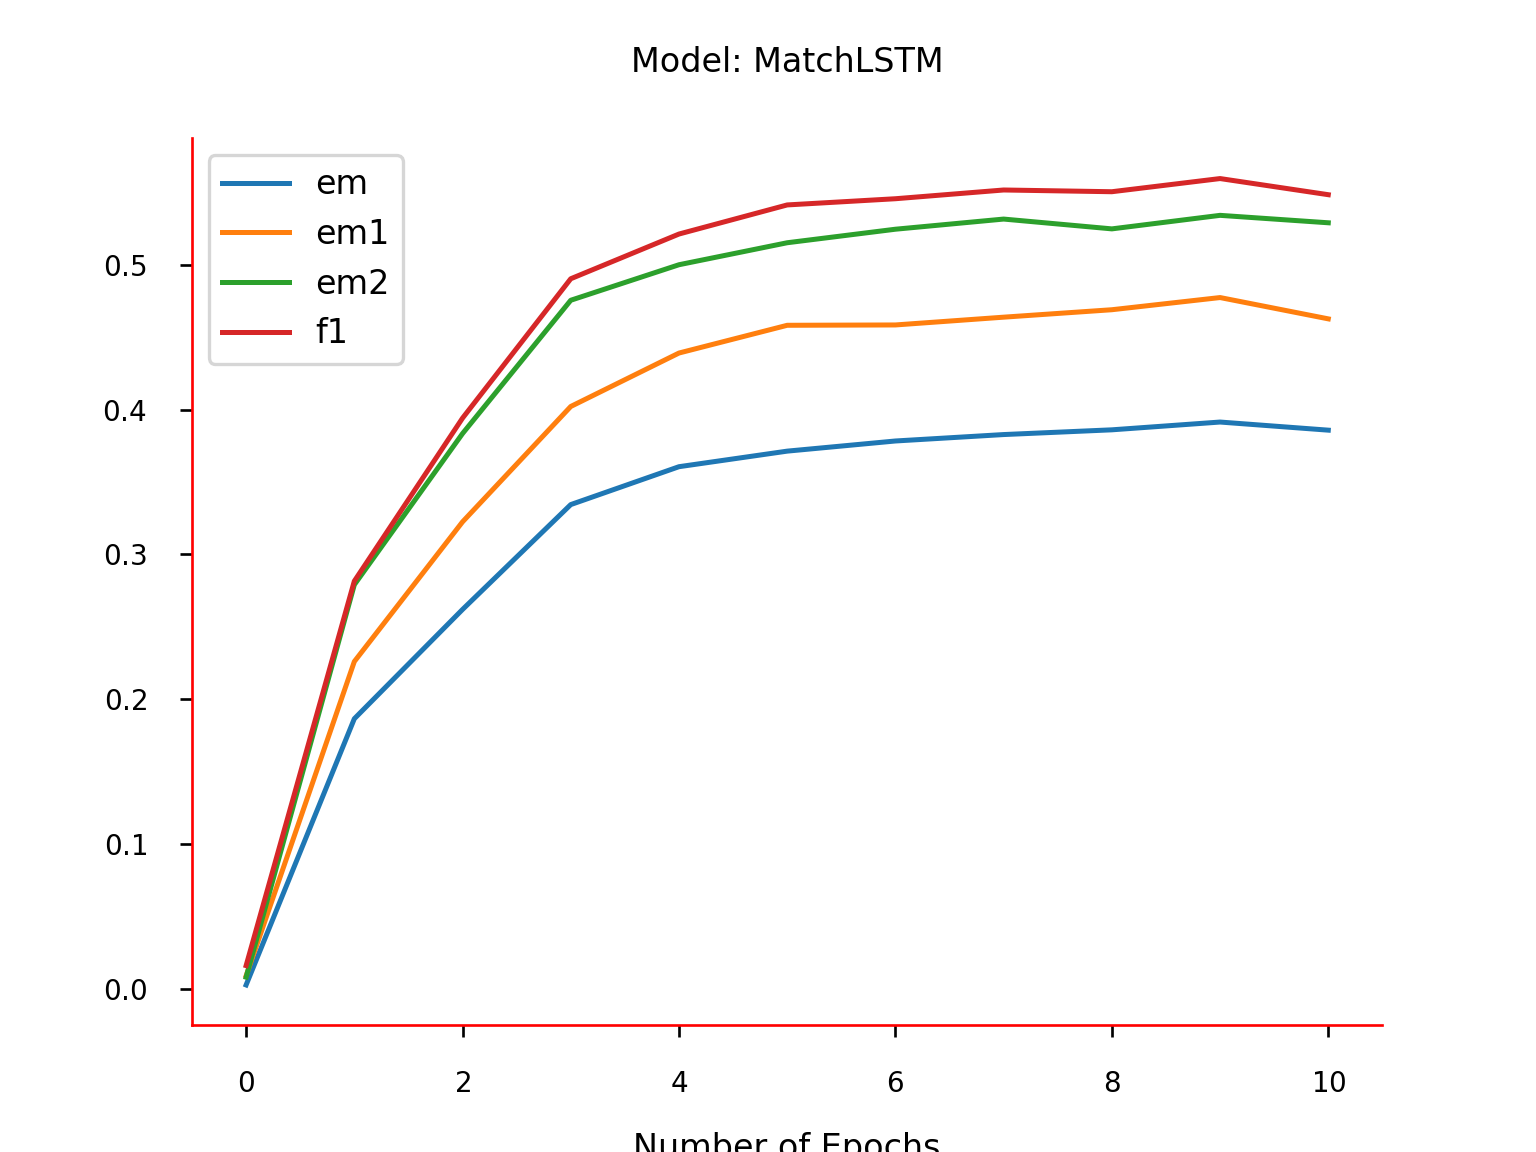
\includegraphics[trim={0 4mm 0 0},clip, width=220px]{includes/plots/match-lstm/accuracy-match-lstm.png}
					\caption*{(a) Match-LSTM}
				\end{minipage}
				\begin{minipage}{0.47\textwidth}

					\centering
					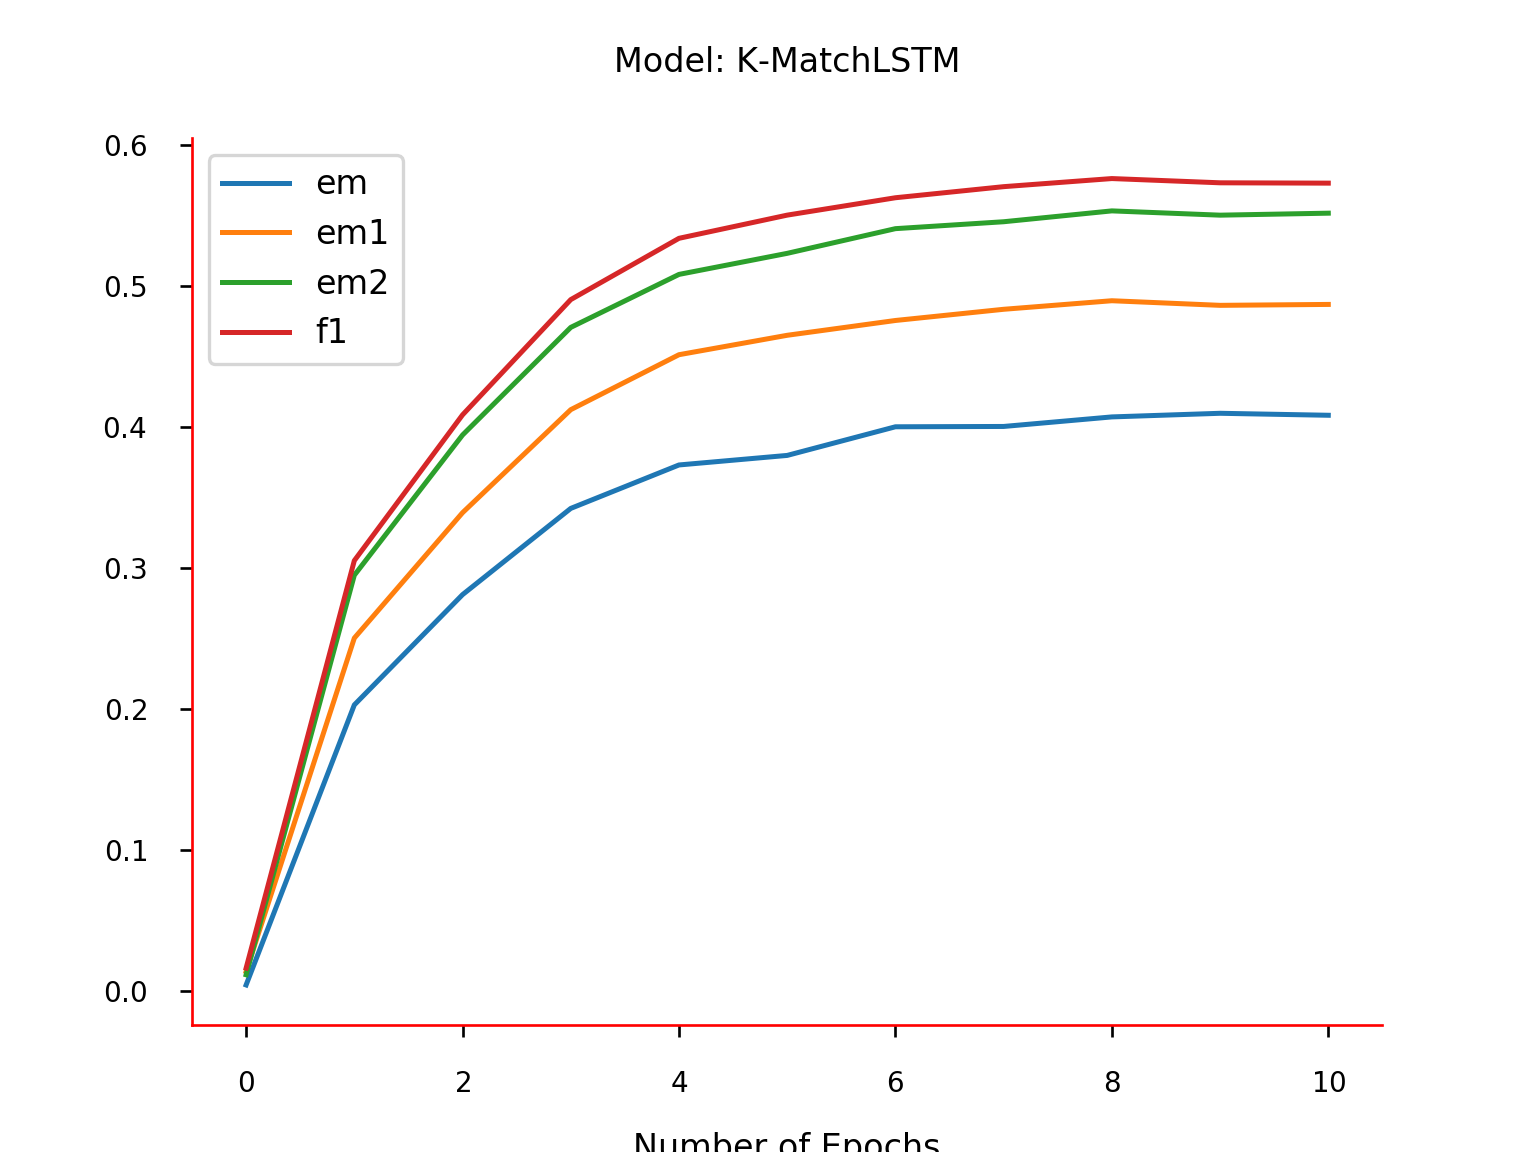
\includegraphics[trim={0 4mm 0 0},clip,width=220px]{includes/plots/match-lstm/accuracy-k-match-lstm.png}
					\caption*{(b) K-Match-LSTM}
				\end{minipage}
				\caption{Accuracy Analysis - Match-LSTM (left) and K-Match-LSTM (right)}
				\label{fig:k-match-comparison}
	\end{figure}
	   Analysis of the efficiency scores in the figure \ref{fig:k-match-comparison} provides an evidence that without any increase in the training time our model performed better in comparison to base model.


	   Another heuristic approach is applied in order to improve the test accuracy Since the loss for start and end tokens is computed individually, we weight each loss with the weights proportional to the inverse of the exact match at that token. This significantly improved the convergence and accuracy.\\
	   The new loss is given as
            \begin{align*}
                - w_1 \cdot \log p(a_s \,|\, \*P_n, \*Q_n) - w_2 \cdot \log p(a_e \,|\, \*P_n, \*Q_n)
            \end{align*}
            where
            \begin{align*}
                w_1 = 2 \frac{em2}{em1 + em2} \quad w_2 = 2 \frac{em1}{em1 + em2}
            \end{align*}

    \begin{figure}[ht!]
		       \begin{minipage}{0.47\textwidth}
					\centering
					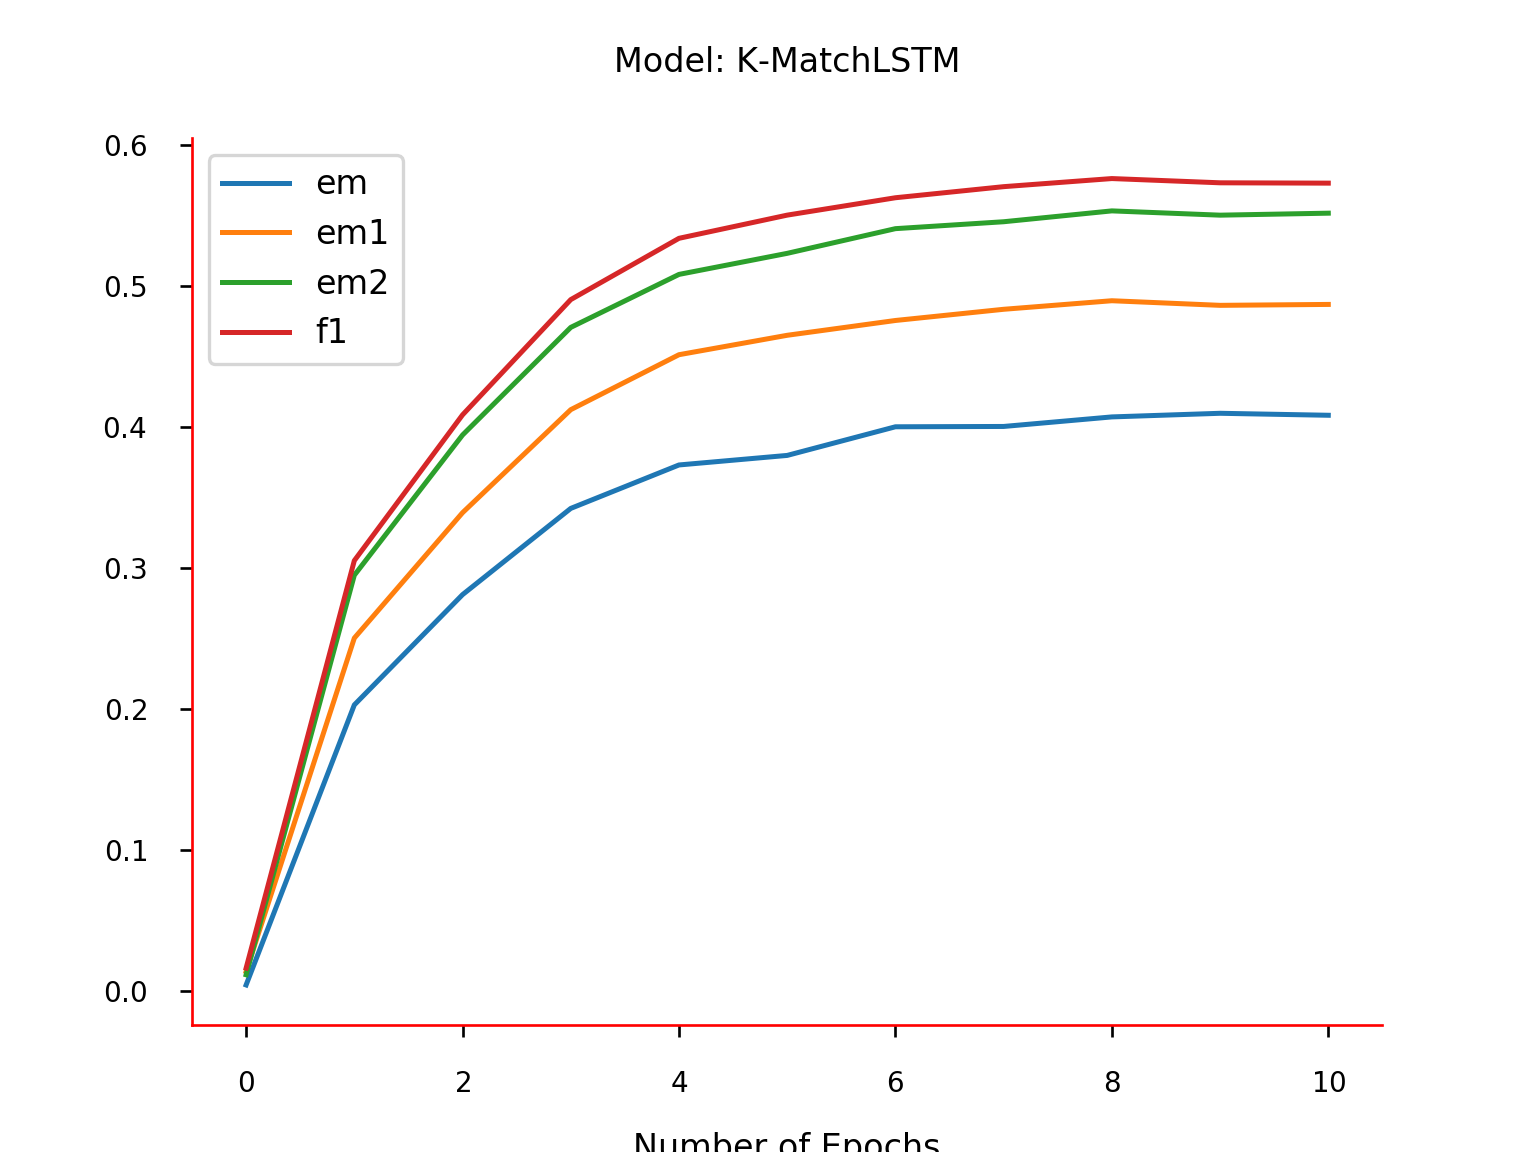
\includegraphics[trim={0 4mm 0 0},clip, width=220px]{includes/plots/match-lstm/accuracy-k-match-lstm.png}
					\caption*{(a) K-Match-LSTM}
				\end{minipage}
				\begin{minipage}{0.47\textwidth}

					\centering
					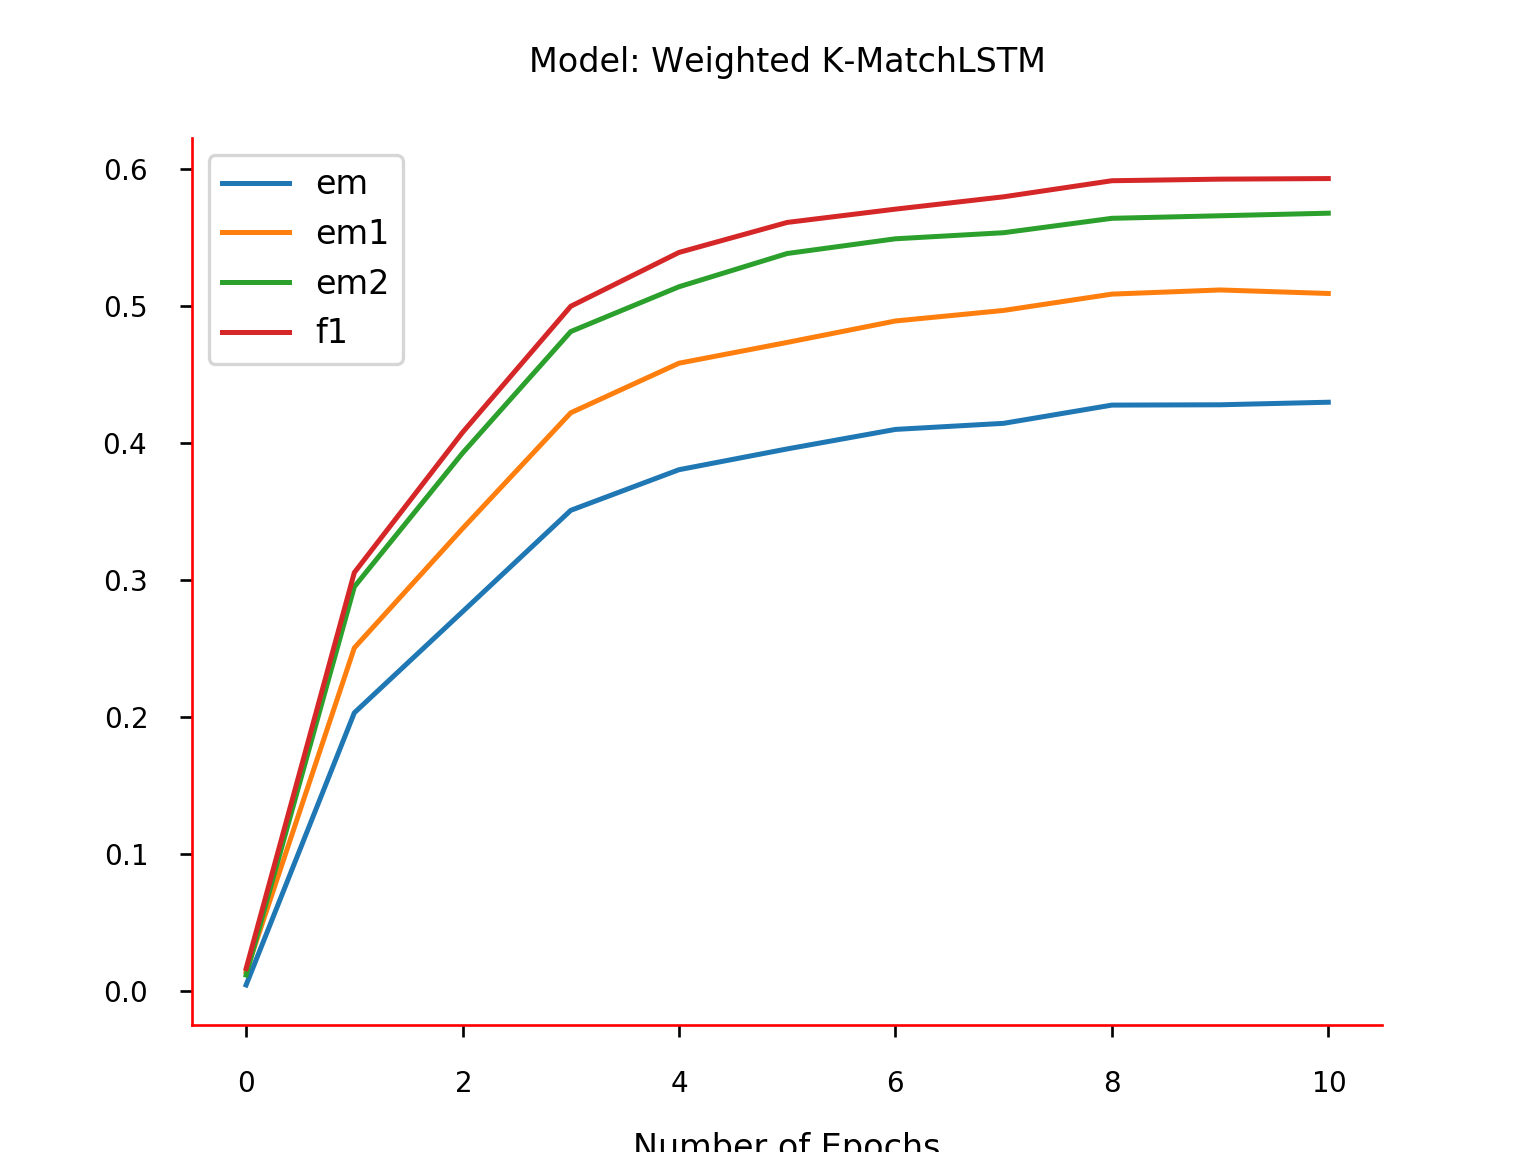
\includegraphics[trim={0 4mm 0 0},clip,width=220px]{includes/plots/match-lstm/accuracy-weighted-k-match-lstm.png}
					\caption*{(b) Weighted-K-Match-LSTM}
				\end{minipage}
				\caption{Accuracy Analysis - K-Match-LSTM (left) and Weighted-K-Match-LSTM (right)}
				\label{fig:weighted-match-comparison}
	\end{figure}
     Further adoption of weighted errors significantly improve the accuracy in terms of various efficiency scores in comparison to K-Match-LSTM as evident from figure \ref{fig:weighted-match-comparison}.


    \begin{figure}[ht!]
		\centering
	    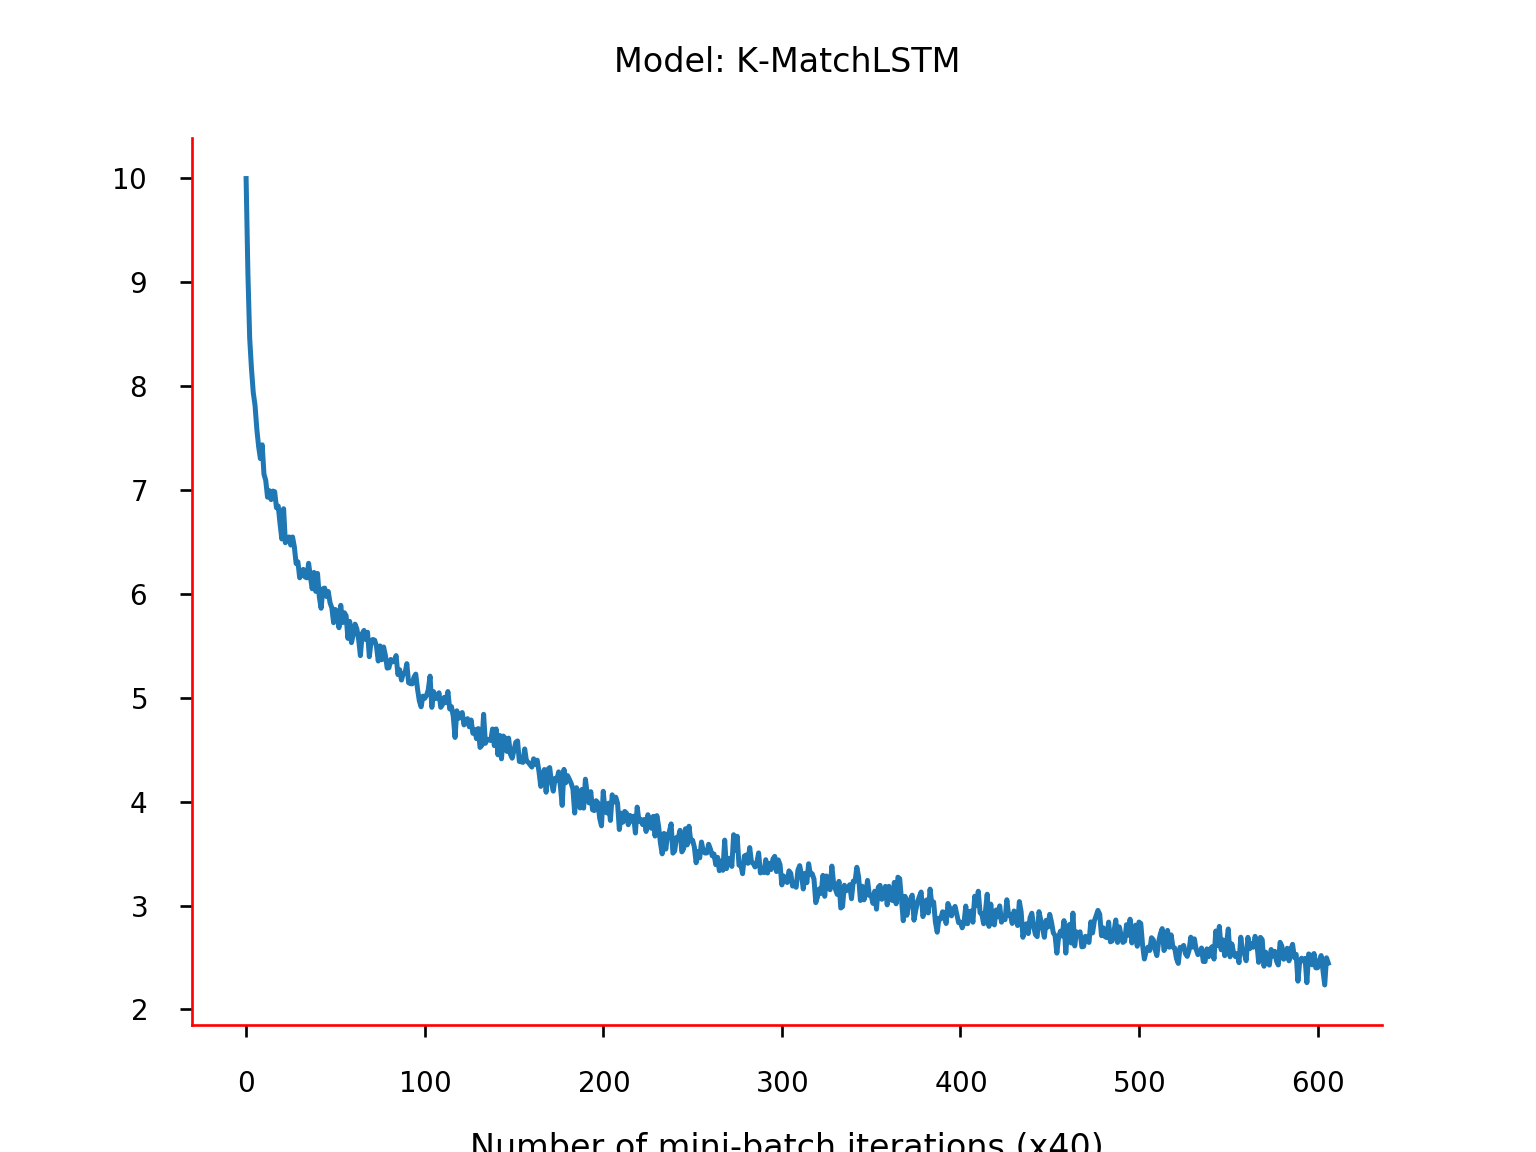
\includegraphics[trim={0 4mm 0   0},clip,width=220px]{includes/plots/match-lstm/loss-k-match-lstm.png}
	    \hspace{5mm}
	    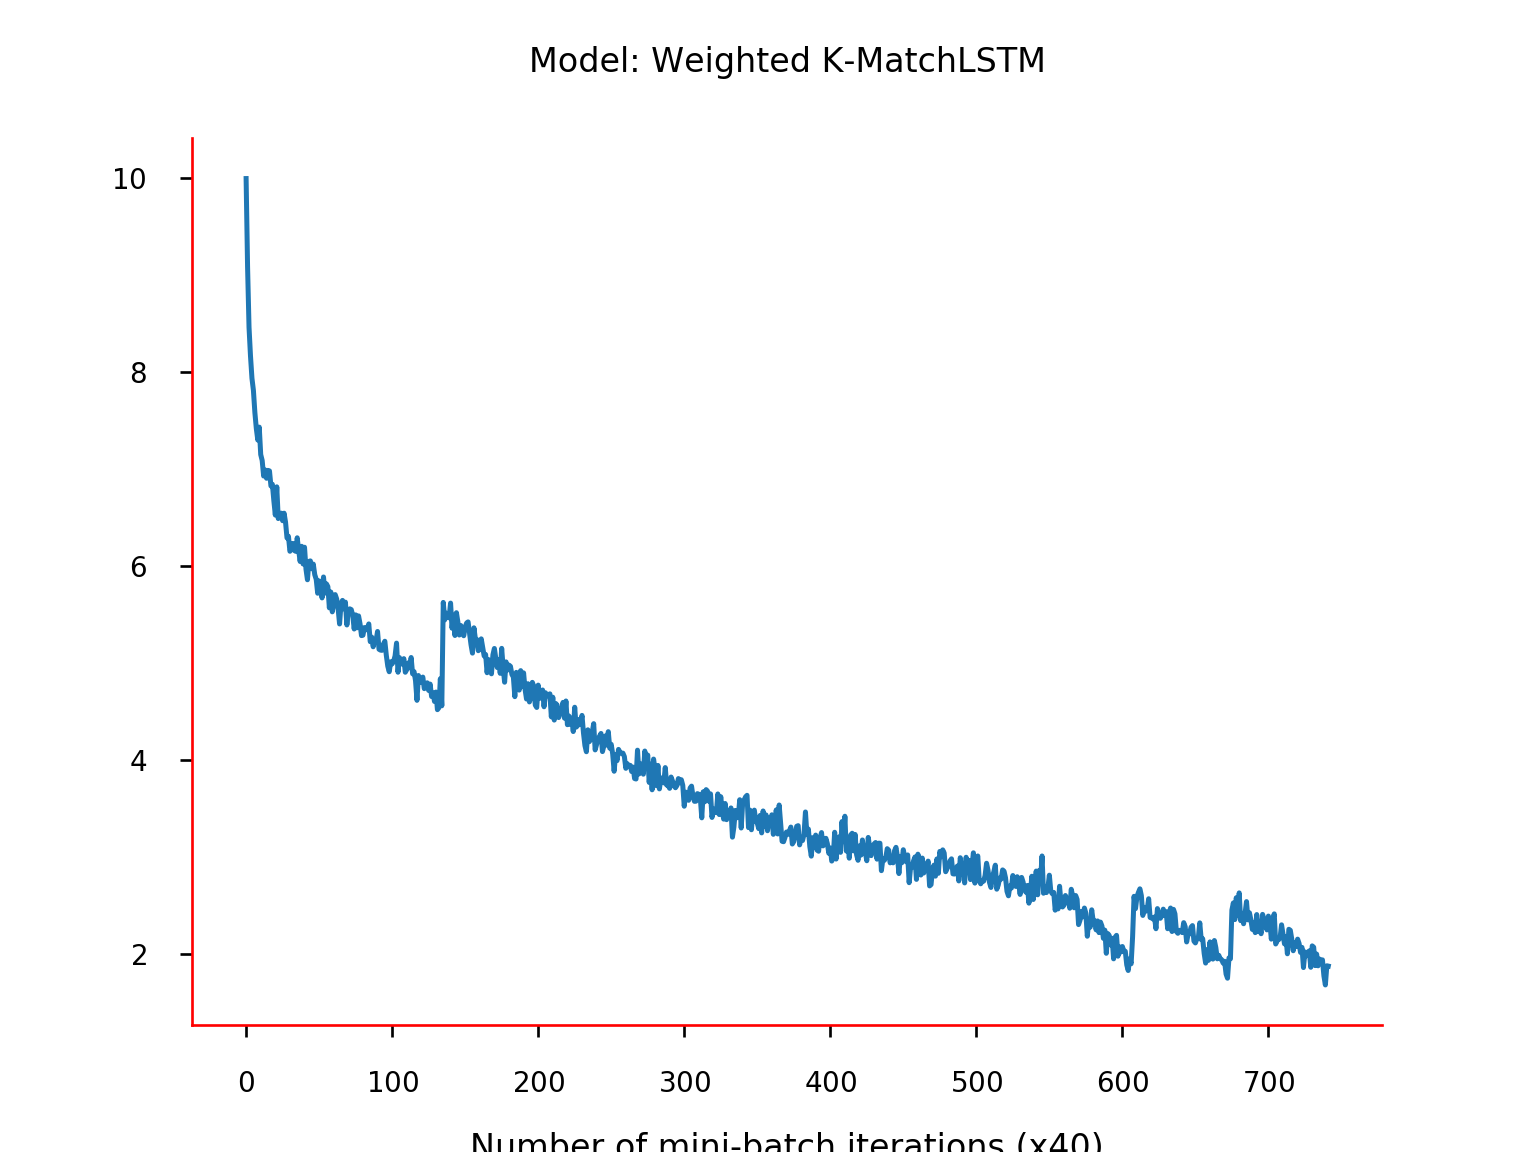
\includegraphics[trim={0 4mm 0 0},clip,width=220px]{includes/plots/match-lstm/loss-weighted-k-match-lstm.png}
		\caption{Convergence analysis for Different Models}
	\end{figure}

	\begin{figure}[ht!]
		\centering
	    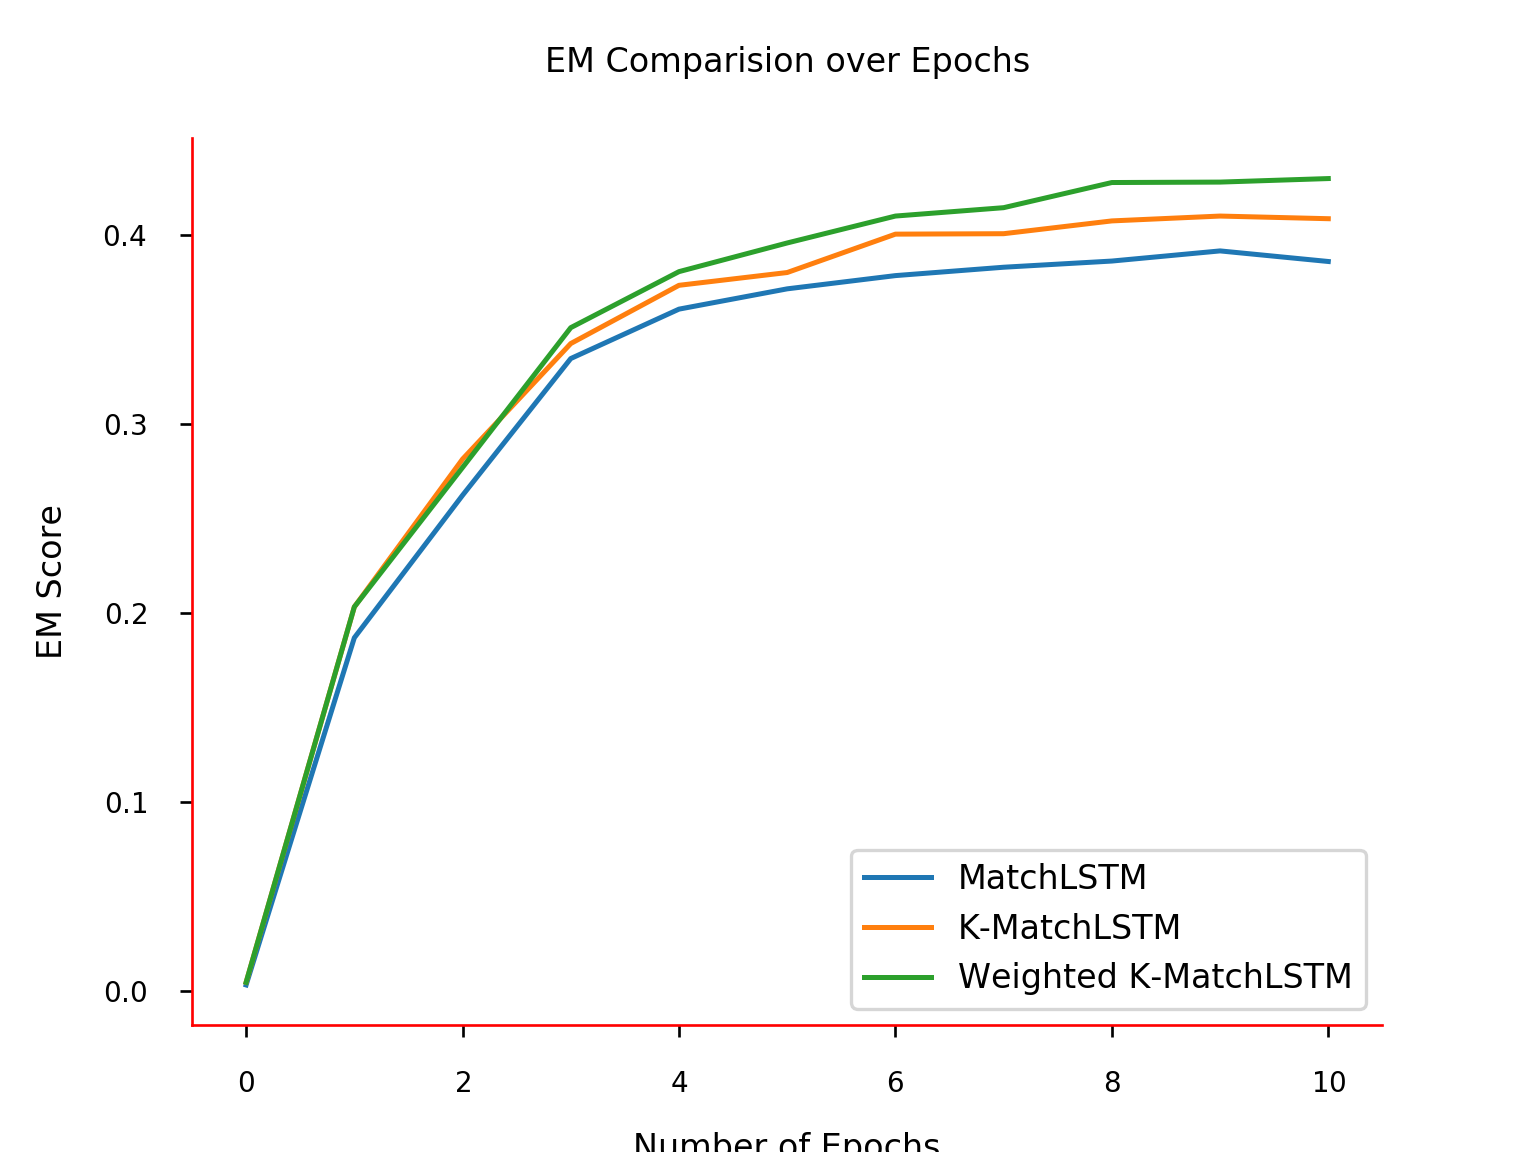
\includegraphics[trim={0 4mm 0 0},clip,height=180px]{includes/plots/match-lstm/comparision.png}
		\caption{EM scores for Different Models}
		\label{em-comparison}
	\end{figure}
	Figure \ref{em-comparison} provides empirical evidence of both weighted and cluster intrinsic model outperforming the base model as the number of epochs become large under some regulation.
\end{psubsection}

\begin{psubsection}{Attention Model}

\tb{Model Description}
Our  model has three components: a \tb{RNN encoder layer}, that encodes both the context and the question into hidden states, \tb{an attention layer}, that combines the context and question representations, and an \tb{output layer}, which applies a fully connected layer and then two separate softmax layers (one to get the start location, and one to get the end location of the answer span).

\tb{RNN Encoder Layer : }For each SQuAD example (context, question, answer), the context is represented by a sequence of d-dimensional word embeddings $\mb{x_1},\dots,\mb{x_N} \in \mathbb{R}^    d$, and the question by a sequence of d-dimensional word embeddings $\mb{y_1},\dots,\mb{y_M}\in \mathbb{R}^d$. These are fixed, pre-trained GloVe embeddings. The embeddings are fed into a 1-layer bidirectional GRU (which is shared between the context and the question):

\begin{align*}
    \{\ora{\mb{c_1}}\ola{\mb{c_1}},\dots,\ora{\mb{c_N}},\ola{\mb{c_N}}\} &= biGRU(\{\mb{x_1},\dots,\mb{x_N}\}) \\
     \{\ora{\mb{q_1}}\ola{\mb{q_1}},\dots,\ora{\mb{q_M}},\ola{\mb{c_M}}\} &= biGRU(\{\mb{y_1},\dots,\mb{y_M}\})
\end{align*}

The bidirectional GRU produces a sequence of forward hidden states $\ora{\mb{c_i}}\in \mathbb{R}^h$ for the context and $\ora{\mb{q_j}}\in \mathbb{R}^h$ for the question) and a sequence of backward hidden states $\ola{\mb{c_i}}$ and $\ola{\mb{q_j}}$. We concatenate the forward and backward hidden states to obtain the context hidden states $\mb{c_i}$ and the question
hidden states $\mb{q_j}$ respectively:

\begin{align*}
    \mb{c_i} & = [\ora{\mb{c_i}},\ola{\mb{c_i}}] \in \mathbb{R}^{2h} \ \forall i \in \{1,\dots,N\}\\
    \mb{q_j} & = [\ora{\mb{q_j}},\ola{\mb{q_j}}] \in \mathbb{R}^{2h} \ \forall i \in \{1,\dots,M\}
\end{align*}

\tb{Attention Layer}
 We used \textbf{ Scaled Dot-Product Attention} and \textbf{Multi-Head Attention} for our task.  Our main  aim was to decrease the training time that the current state of art model takes and provide at par accuracy. We were pretty successful in decreasing the training time to 20 min for 1 epoch and model took 20 epoch to reach it's maxima.  For the further discussion, we have denoted keys as the context hidden states and the values as the question hidden states.

\begin{frame}{}
    \begin{figure}[ht!]
		\centering
	    \includegraphics[trim={0 4mm 0 0},clip,height=200px]{includes/nlp.png}
		\caption{Overview of second Model}
	\end{figure}
\end{frame}

 \begin{subsubsection}{Scaled Dot-Product Attention}
      This attention mechanism was proposed in ~cite{Vaswani et al. 2017}, in involves multiple heads each of which first linearly down-projects the keys and the values to a lower dimensional space and computes a standard attention between them. The output across the head is then concatenated. The benefits of this approach lie in its ability to compute attention from various perspectives and its also benefits from parallelizability.

       \begin{figure}[ht!]
			\centering
			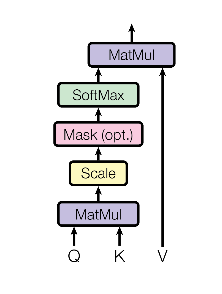
\includegraphics[height=100px]{includes/Attention-Dot.png}
			\caption{Scaled Dot-Product Attention. \et{\citep[Source:][]{attention}}}
			\label{fig:attention-dot}
		\end{figure}

      The input consists of queries and keys of dimension $d_k$, and values of dimension $d_v$. We compute the dot products of the query with all keys, divide each by $\sqrt{d_k}$, and apply a softmax function to obtain the weights on the values. In practice, we compute the attention function on a set of queries simultaneously,  packed together into a matrix $Q$. The keys and values are also packed together into matrices $K$ and $V$. We compute the matrix of outputs as:
      $$Attention(\*Q, \*K, \*V ) = softmax\Big(\frac{\*Q\*K^T}{\sqrt{d_k}}\Big)V$$
      The two most commonly used attention functions are additive attention [2], and dot-product (multiplicative)
      attention. Dot-product attention is identical to our algorithm, except for the scaling factor of $\frac{1}{\sqrt{d_k}}$. Additive attention computes the compatibility function using a feed-forward network with
      a single hidden layer. While the two are similar in theoretical complexity, dot-product attention is
      much faster and more space-efficient in practice, since it can be implemented using highly optimized
      matrix multiplication code. While for small values of $d_k$ the two mechanisms perform similarly, additive attention outperforms dot product attention without scaling for larger values of $d_k$ [3]. We suspect that for large values of
      $d_k$, the dot products grow large in magnitude, pushing the softmax function into regions where it has
      extremely small gradients [4]. To counteract this effect, we scale the dot products by $\frac{1}{\sqrt{d_k}}$

 \end{subsubsection}

 \begin{subsubsection}{Multi-Head Attention}
     Instead of performing a single attention function with $d_{model}$-dimensional keys, values and queries, we found it beneficial to linearly project the queries, keys and values $h$ times with different, learned linear projections to $d_k$, $d_k$ and $d_v$ dimensions, respectively.

        \begin{figure}[ht!]
			\centering
			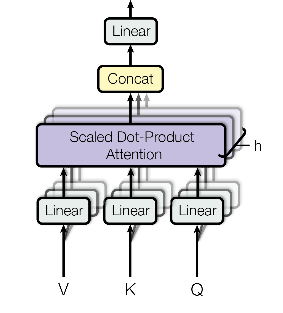
\includegraphics[height=100px]{includes/Attention-Multi.png}
			\caption{Multi-Head Attention. \et{\citep[Source:][]{attention}}}
			\label{fig:attention-dot}
		\end{figure}

     On each of these projected versions of queries, keys and values we then perform the attention function in parallel, yielding $d_v$-dimensional output values. These are concatenated and once again projected, resulting in the final values, as depicted in Fig.
     Multi-head attention allows the model to jointly attend to information from different representation sub spaces at different positions. With a single attention head, averaging inhibits this.

     \begin{align*}
       MultiHead(\*Q, \*K, \*V ) &= Concat(head_1, ..., head_h)\*W^O  \\
      where \ head_i & = Attention(\*Q\*W^Q, \*K\*W_i^K, \*V\*W_i^V)
     \end{align*}

    Where the projections are parameter matrices $\*W_i^Q \in \mathbb{R}^{d_{model}\times d_k}$, $\*W_i^K \in \mathbb{R}^{d_{model}\times d_k}$, $\*W_i^V \in \mathbb{R}^{d_{model}\times d_k} \\ \text{and \ } \*W^O \in \mathbb{R}^{hd_v \times d_{model}}$.
    In this work we employ $h = 8$ parallel attention layers, or heads. For each of these we use $d_k = d_v = d_{model}/h = 64$. Due to the reduced dimension of each head, the total computational cost is similar to that of single-head attention with full dimensionality.

 \end{subsubsection}

\tb{Output Layer}: Next, each of the blended representations $\mb{b_i}$ are fed through a fully connected layer followed by a ReLU non-linearity:

$$\mb{b_i`} = ReLU(\mb{W}_{FC}\mb{b_i} + \mb{v}_{FC})\in \mathbb{R}^h \ \forall i \in \{1,\dots,N\}$$

where $\mb{W}_{FC} \in \mathbb{R}^{h \times 4h}$ and $\mb{v}_FC \in \mathbb{R}^h$ are a weight matrix and bias vector. Next, we assign a score (or logit) to each context location $i$ by passing $\mb{b_i`}$ through a downprojecting linear layer:

$$logits_i^{start} = \mb{W^T_{start}}\mb{b`_i} + u_{start} \ \in \mathbb{R} \ \forall i \in \{1,\dots,N\}$$

where $\mb{w}_{start} \in \mathbb{R}^h$ is a weight vector and $u_{start}\in \mathbb{R} is a bias term$. Finally, we apply the softmax
function to $logits_{start} \in \mathbb{R}^N$ to obtain a probability distribution $p_{start} \in \mathbb{R}^N$ over the context
locations $\{1,\dots,N\}$:

$$p^{start} = softmax(logits^{start}) \in \mathbb{R}^N$$

We compute a probability distribution $p^{end}$ in the same way (though with separate weight $\mb{w}_{end}$ and $u_{end}$).

\tb{Loss : } Our loss function is the sum of the cross-entropy loss for the start and end locations. That is, if the gold start and end locations are $i_{start} \in \{1,\dots,N\}$ and $i_{end} \in \{1,\dots,N\}$ respectively, then the loss for a single example is:

$$loss = -\log p^{start} (i_{start})-\log p^{end}(i_{end})$$

During training, this loss is averaged across the batch and minimized with the Adam optimizer.

\tb{Prediction : }At test time, given a context and a question, we simply take the argmax over $p^{start}$ and $p^{end}$ to obtain the prediction span $(l^{start},l^{end})$:

\begin{align*}
    l^{start} &= \underset{i \in \{1,\dots,N\}}{argmax} \ p_i^{start}\\
    l^{end} &= \underset{i \in \{1,\dots,N\}}{argmax} \ p_i^{end}
\end{align*}
\end{psubsection}

\end{psection}

\begin{psection}{Results}
The model was trained for 20 epochs with around \textbf{20 min} training time of each epoch.The addition of Multihead attention resulted in improvement of F1 score by 5\% which is significant.Other major improvement came from using forward and backward lstm, using the length of embedding found out from data analysis, using mask to prevent model from iterating on padding.
	\begin{table}[ht!]
			\centering
			\begin{tabular}{l@{\hspace{1em}}|cc|cc}
				\multirow{2}{*}{\bt{Model}}	&	\multicolumn{2}{c|}{\bt{Training Set}}	&	\multicolumn{2}{c}{\bt{Test Set}}	\\
											&	\bt{EM} & \bt{F1}						&	\bt{EM} & \bt{F1}					\\
				\hline
				Stanford Baseline 	& -	 & -		&	34.4 & 43.9							\\
				Stanford Baseline LSTM 			&	- & -								&	35.3 & 44.9							\\
				MultiHead Attention  			 & 67.5	&	80								 & 45.95	& 60.05				\\
				\end{tabular}
			\caption{Result Obtained on Multi Head Attention against baseline squad model by stanford  \et{\citep[Source:][]{r-net}}}
			\label{tab:models}
		\end{table}

   \begin{figure}[ht!]
		\centering
	    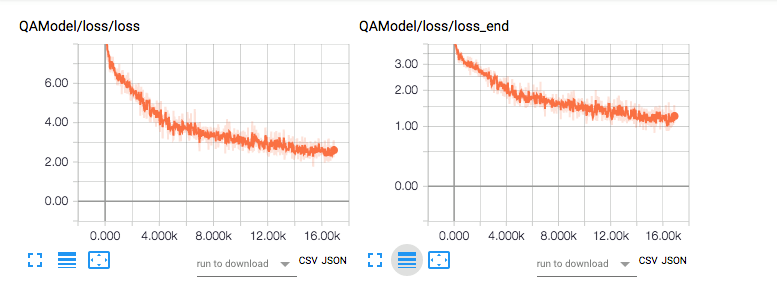
\includegraphics[trim={0 4mm 0 0},clip,height=100px]{includes/30698020_1243260699138580_809976629538324480_n.png}
		\caption{Model Loss}
	\end{figure}
   \begin{figure}[ht!]
		\centering
	    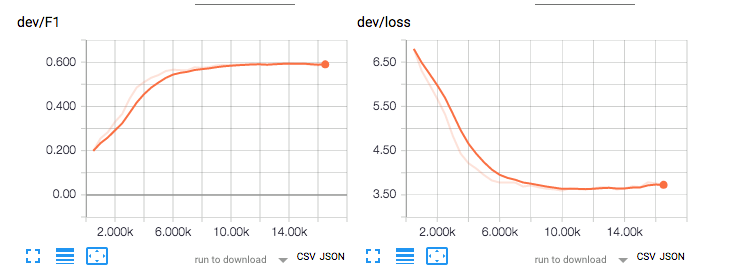
\includegraphics[trim={0 4mm 0 0},clip,height=100px]{includes/30656704_1243260925805224_9155158550215917568_n.png}
		\caption{F1 score and loss}
	\end{figure}
   \begin{figure}[ht!]
		\centering
	    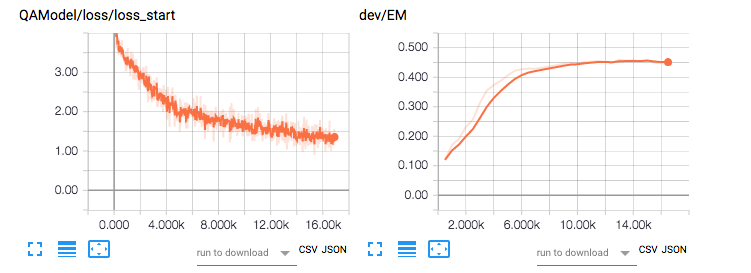
\includegraphics[trim={0 4mm 0 0},clip,height=100px]{includes/30656669_1243260725805244_6970738131930710016_n.png}
		\caption{EM score and loss}
	\end{figure}


\end{psection}
\begin{psection}{Analysis}
The major difference in EM and F1 score is because of imprecise boundaries. This may be due to ambiguity in questions and answers provided in squad as the dataset is labeled by humans. Fig 19 shows one such case.Also the model is trained to answer to focus on "What" , "Who", "When" ,"How" phrases rather than understanding technicalities of questions like comparing with adverbial phrases like greatest, biggest, one among the following etc.

 \begin{figure}[ht!]
	    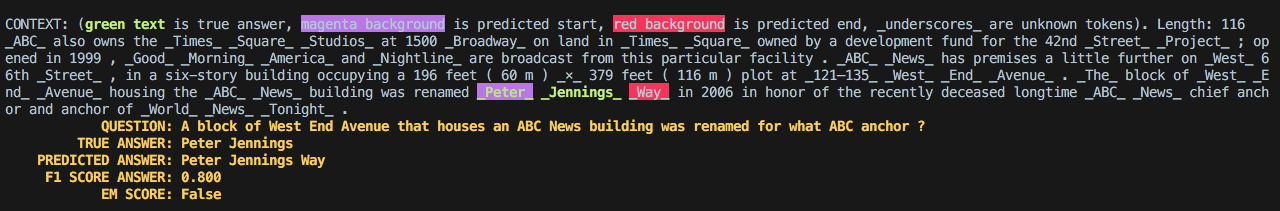
\includegraphics[trim={0 4mm 0 0},clip,height=100px]{includes/2.png}
		\caption{Controversial example showing difference in EM and F1}
	\end{figure}

\end{psection}

\begin{psection}{Future extension}
One idea for further improvement as proposed by Ryan Almodovar that we can use  is to build questions summaries.It is conceivable that adding paragraph summaries to each question word would also be helpful in relating the paragraph to the question. One could compute the expected paragraph vector for each question word in the same way that we did the reverse, and augment the questions vectors with this information.

\end{psection}
\bibliography{proposal}
\bibliographystyle{plainnat}
\begin{psection}{Contribution}
All group memebers did equal amount of work ie each 16.7\%
\end{psection}
\end{document}
